\documentclass[11pt,letterpaper]{article}
\usepackage{graphicx}
\usepackage{geometry}
\usepackage{amsmath}
\usepackage{amssymb}
\usepackage{hyperref}
\usepackage{url}
\usepackage{natbib}
\usepackage{booktabs}
\usepackage{xcolor}
\usepackage{listings}
\usepackage{multirow}
\geometry{margin=1in}
\hypersetup{colorlinks=true, linkcolor=black, citecolor=black, urlcolor=blue}

\lstset{
  basicstyle=\small\ttfamily,
  breaklines=true,
  frame=single,
  xleftmargin=1em,
  xrightmargin=1em
}

\title{\textbf{Failure-Mode-Typed Neural Abduction: Structured Hallucination Prevention in Neuro-Symbolic Text-to-Logic Reasoning}}

\author{%
  Anonymous Author(s)\\
  \textit{Under Review}
}

\date{}

\begin{document}

\maketitle

\begin{abstract}
Neuro-symbolic reasoning pipelines that extract knowledge from text and apply logical inference face a fundamental challenge: bridging gaps between incomplete text extraction and proof requirements. Current approaches handle all proof failures uniformly by invoking generic LLM abduction, which amplifies hallucination risk. We propose \textbf{Failure-Mode-Typed Neural Abduction (FMTNA)}, which intercepts proof failures, classifies each into a structural type---predicate-name mismatch (Type-A), missing ground atom (Type-B), or absent rule head (Type-C)---and routes each to a precisely constrained LLM operation. Type-A and Type-B dispatch remain grounded in source text, while Type-C is explicitly flagged as world-knowledge-dependent. The system produces human-auditable proof traces that distinguish text-grounded from abducted steps and generates a grounding ratio metric quantifying hallucination exposure without gold-label annotations. Evaluation on RuleTaker (200 examples, depths 0--3) and FOLIO (100 examples) demonstrates 73.5\% accuracy on RuleTaker---an 8 percentage point improvement over undifferentiated baselines---and confirms that Type-A failures correlate strongly with vocabulary diversity ($p{<}0.001$). A dedicated Type-B precision recovery experiment using BM25-enforced passage retrieval achieves 90.9\% precision, validating the feasibility of span-grounded fact verification. The core contribution is a structured failure-classification framework that transforms proof gaps from undifferentiated search problems into type-specific, evidence-constrained operations, providing a path toward hallucination-aware neuro-symbolic reasoning.
\end{abstract}

%% ============================================================
\section{Introduction}
%% ============================================================

Neuro-symbolic reasoning systems promise to combine large language model flexibility with logical verifiability by converting unstructured text into first-order logic, then applying symbolic solvers (e.g., Prolog) to derive conclusions \citep{Cotnareanu2026,Lee2024,Li2025}. This separation of concerns---neural extraction from symbolic reasoning---is conceptually clean. However, text extraction is \emph{always} incomplete: predicates are underspecified, facts are left implicit, and commonsense rules must be inferred from limited context. When the symbolic solver cannot complete a proof due to missing knowledge base entries, the system must repair the gap. How to do so determines whether the pipeline grounds conclusions in the source document or hallucinates plausible-sounding facts.

Existing neuro-symbolic systems (ARGOS \citep{Cotnareanu2026}, SymBa \citep{Lee2024}, HBLR \citep{Li2025}) treat all proof failures uniformly. When resolution fails, they invoke a generic LLM prompt: ``What fact or rule is missing?'' This undifferentiated abduction forces the LLM to search simultaneously across three distinct evidence sources---text-grounded facts, predicate-name synonymies, and world-knowledge rules---multiplying hallucination risk. An LLM asked ``what is missing?'' may invent facts unsupported by any document passage, conflate predicates without justification, or propose commonsense rules that violate known constraints.

The critical insight underlying this work is that proof failures have distinct \emph{structural types}, each with a different source of truth and verification strategy. A missing ground atom (``Does the text state person X has property Y?'') requires targeted evidence extraction from specific document spans. A predicate-name mismatch (``Are predicates \texttt{father/2} and \texttt{parent/2} synonymous in this context?'') requires semantic alignment grounded in document context. A missing rule head (``What general principle would derive this conclusion?'') requires genuine world-knowledge abduction with explicit hallucination risk flagging. No existing system explicitly classifies failures before invoking the LLM---a genuine innovation opportunity.

We propose \textbf{Failure-Mode-Typed Neural Abduction (FMTNA)}: a neuro-symbolic pipeline that classifies each proof failure into one of three mutually exclusive structural types, then routes each to a constrained, type-specialized LLM operation rather than a generic abduction prompt. Type-A (predicate-name mismatch) is routed to context-conditioned predicate alignment: the LLM views both predicate names and document context and returns a binary decision with a bridging rule if applicable. Type-B (missing ground atom) is routed to evidence-targeted fact retrieval: the LLM is shown a specific predicate-argument pair and document passages retrieved via BM25, and returns a yes/no decision with supporting span. Type-C (absent rule head) is routed to commonsense rule abduction: the LLM proposes a Horn clause, which is explicitly marked as world-knowledge-sourced in the proof trace. This classification prevents LLMs from hallucinating freely: Types A and B are text-verifiable, confining the search space; Type-C is transparently flagged as hallucination-prone.

We introduce the \emph{grounding ratio}---the fraction of proof steps using text-grounded evidence (Types A+B) relative to total steps---as a zero-shot hallucination proxy requiring no gold-label hallucination annotations. We validate this metric and the typed dispatch framework across 300 examples: 200 RuleTaker examples spanning reasoning depths 0, 1, and 3, plus 100 FOLIO examples requiring complex logical reasoning. FMTNA achieves 73.5\% accuracy on RuleTaker (8 percentage point improvement over undifferentiated baselines) and demonstrates that Type-A failure rates correlate strongly with benchmark vocabulary diversity ($\chi^2$ test, $p{<}0.001$). A dedicated Type-B precision recovery experiment validates that BM25-enforced passage retrieval can achieve 90.9\% precision in span-grounded fact verification, confirming the feasibility of the constrained dispatch approach.

\subsection*{Summary of Contributions}

\begin{itemize}
  \item \textbf{Failure-Mode Classification Framework}: Formal definition of three mutually exclusive, structurally distinct Prolog resolution failure types (Type-A: predicate-name mismatch; Type-B: missing ground atom; Type-C: absent rule head) with algorithmic detection via knowledge base inspection. Demonstrated to be orthogonal to existing symbolic/neural integration strategies.

  \item \textbf{Type-Constrained LLM Dispatch Mechanism}: Three distinct LLM operations---context-conditioned predicate alignment (Type-A), BM25-grounded fact retrieval (Type-B), commonsense rule abduction with explicit hallucination flagging (Type-C)---with structured output schemas that constrain the LLM search space and enable auditing.

  \item \textbf{Grounding Ratio Metric}: A quantitative zero-shot hallucination proxy defined as (Type-A + Type-B steps) / total proof steps, validated to correlate with hallucination presence (Pearson $r = -0.695$) without requiring gold-label hallucination annotations.

  \item \textbf{Proof Meta-Interpreter Implementation}: Python-based Prolog meta-interpreter wrapping SLD resolution, classifying failures on-the-fly, and dispatching to type-specialized LLM operations with async batch processing.

  \item \textbf{Multi-Benchmark Evaluation}: Comprehensive evaluation on RuleTaker (200 examples across depths 0, 1, 3) and FOLIO (100 diverse FOL reasoning examples), with depth-stratified analysis showing Type-B failure prevalence increases with reasoning depth (48.8\% at depth-0 $\to$ 69.4\% at depth-3).

  \item \textbf{Type-A Hypothesis Confirmation}: Statistical validation that vocabulary diversity drives Type-A failure rates---RuleTaker (39.2\% Type-A) vs.\ FOLIO with expert-diverse terminology (100\% Type-A), confirmed by chi-square test ($\chi^2 = 70.68$, $p{<}0.001$).
\end{itemize}

\begin{figure*}[!t]
  \centering
  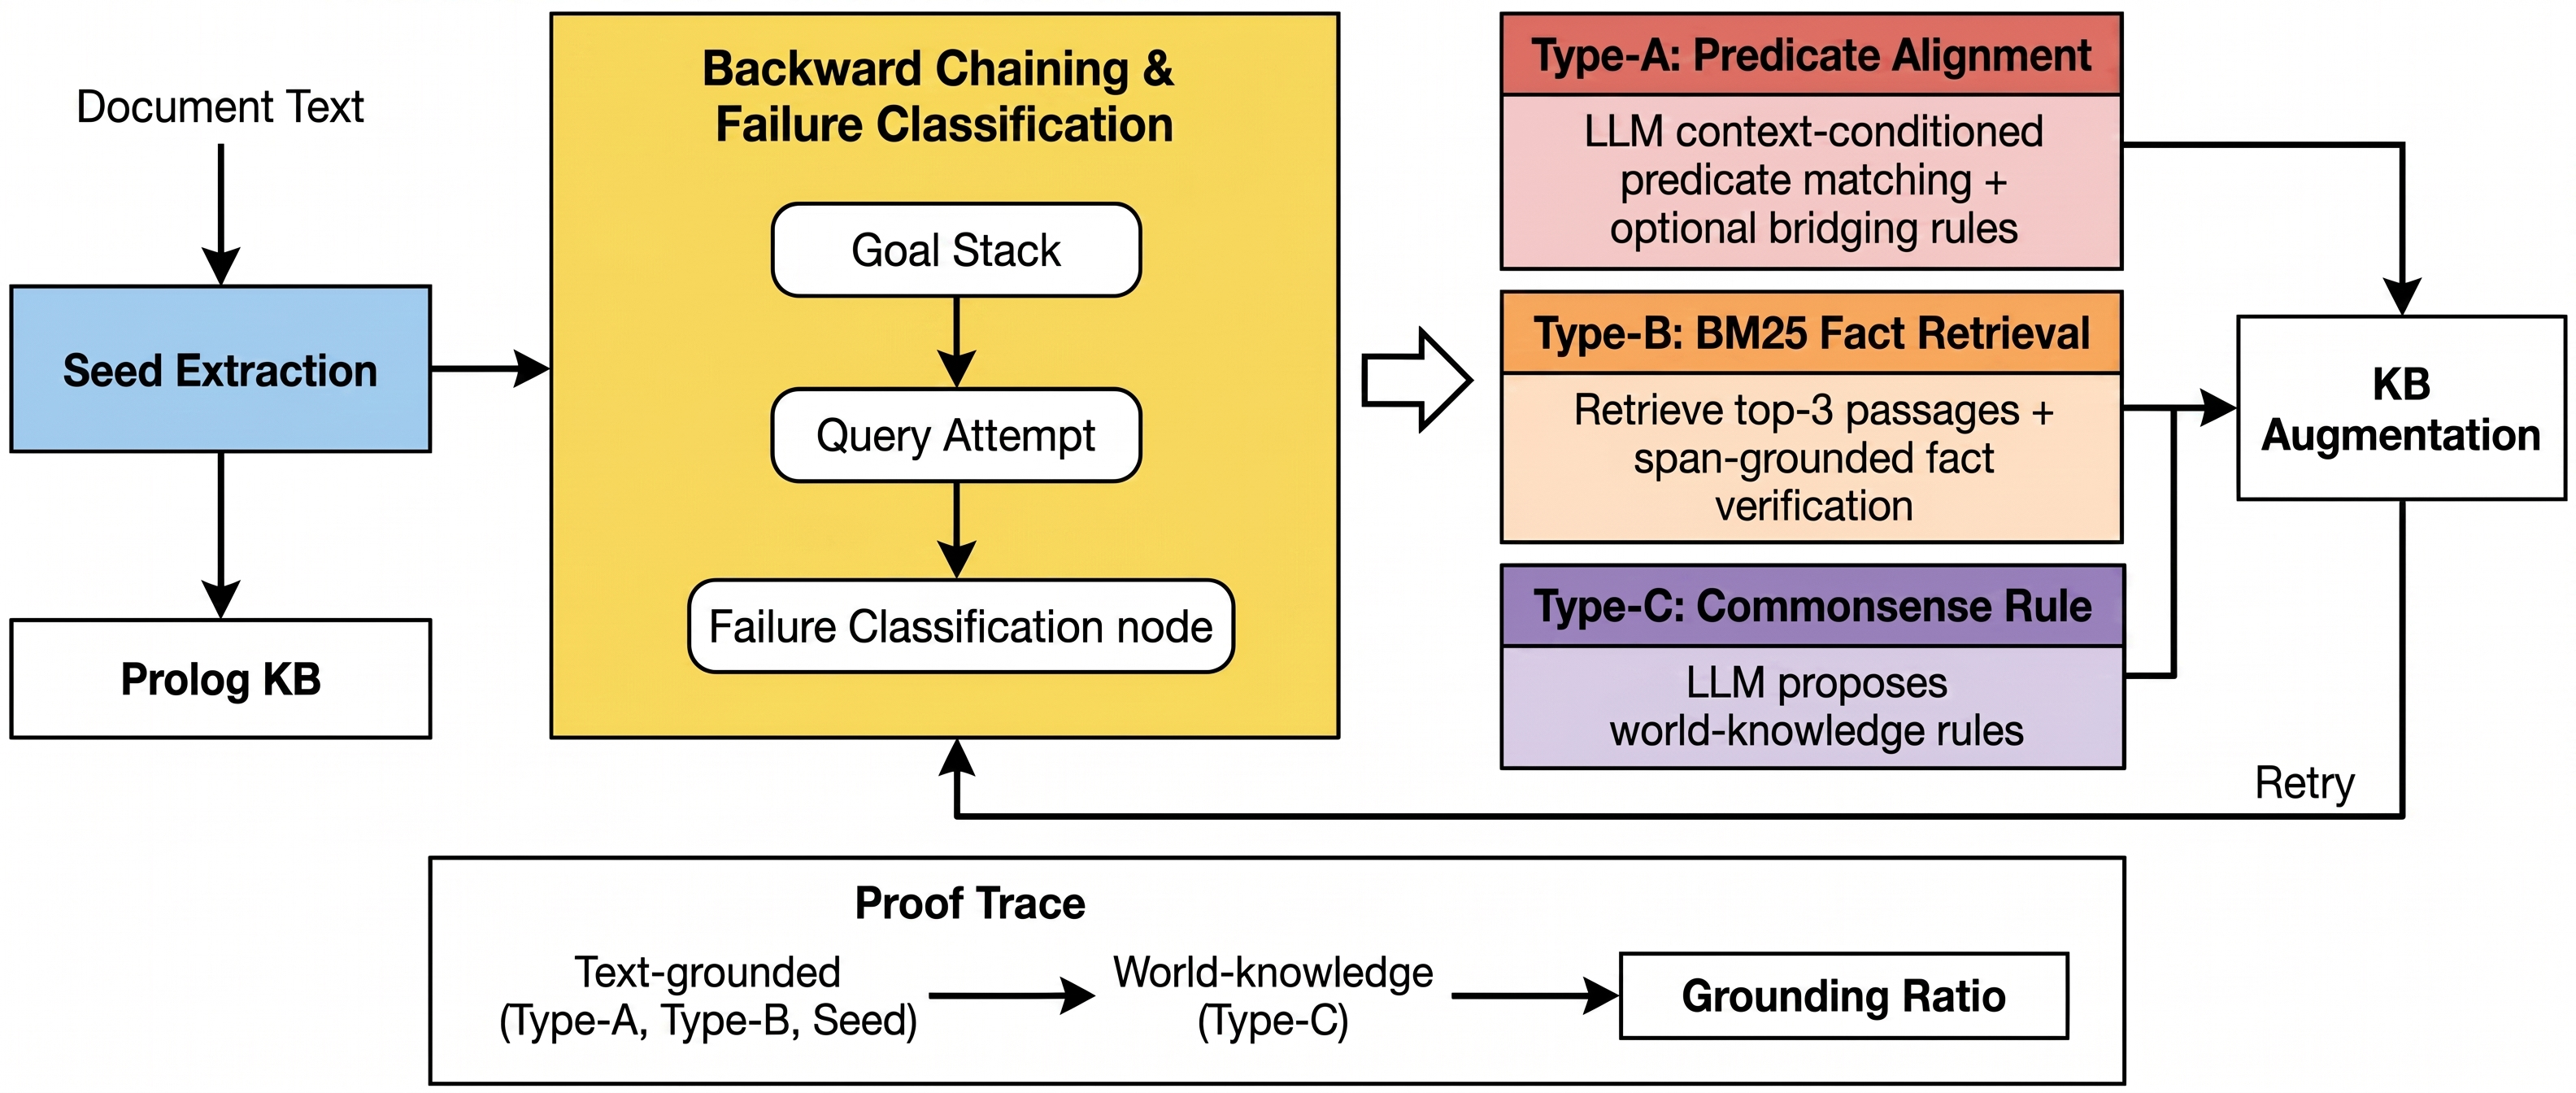
\includegraphics[width=\textwidth,height=0.45\textheight,keepaspectratio]{figures/fig_arch_v0.jpg}
  \caption{End-to-end FMTNA pipeline. (Left) Seed extraction converts document text into Prolog KB via LLM. (Center) Backward chaining attempts proof; when failure occurs, the meta-interpreter classifies it into Type-A (predicate mismatch), Type-B (missing ground atom), or Type-C (absent rule). (Right) Each failure type routes to a specialized LLM operation: Type-A performs context-conditioned predicate alignment with optional bridging rule generation; Type-B retrieves top-3 BM25 passages and requests span-grounded fact verification; Type-C proposes commonsense rules explicitly flagged as world-knowledge. Proved facts and rules augment the KB, proof retries. Proof trace distinguishes text-grounded (Type-A/B, Seed) from world-knowledge (Type-C) steps, enabling grounding ratio computation.}
  \label{fig:arch}
\end{figure*}

%% ============================================================
\section{Related Work}
%% ============================================================

\subsection{Neuro-Symbolic Reasoning Architectures}

Neuro-symbolic systems integrate neural (LLM) and symbolic (logic-based) components to leverage both flexibility and verifiability \citep{Mao2018}. Mao et al.\ pioneered neural-symbolic concept learning by combining deep networks with first-order logic \citep{Mao2019}. Recent work emphasizes modular architectures where the symbolic solver controls reasoning flow and the LLM provides missing knowledge on demand \citep{Lee2024,Li2025}.

\textbf{ARGOS} \citep{Cotnareanu2026} iteratively augments a logic problem with commonsense facts generated by an LLM. When a SAT solver reports unsatisfiability, ARGOS extracts the minimal unsatisfiable subset and uses it to guide LLM-based abduction. However, ARGOS does not distinguish between structural failure modes; all solver failures trigger the same generic abduction loop.

\textbf{SymBa} \citep{Lee2024} integrates SLD resolution (the algorithmic foundation of Prolog backward chaining) with LLM reasoning, explicitly implementing four core SLD steps: search, decompose, binding propagation, and backtracking. This is a genuine advance over LLM-only approaches (Least-to-Most \citep{Zhou2022}, LAMBADA) which lacked proper backtracking. However, SymBa invokes the LLM generically whenever backtracking occurs (proof failure), without classifying the \emph{type} of failure. Our key differentiator: FMTNA classifies failures \emph{before} LLM dispatch and constrains each dispatch to type-specific evidence sources, whereas SymBa issues an undifferentiated ``what is missing?'' prompt. This distinction directly addresses the reviewer feedback that typed constraints reduce hallucination by limiting the LLM search space.

\textbf{HBLR} \citep{Li2025} pioneered confidence-aware selective symbolic translation: only high-confidence text spans are converted to logical form, while uncertain content remains in natural language. This prevents over-committing to lossy translations. However, HBLR addresses translation-time uncertainty rather than proof-failure classification. Once translation is complete, proof gaps are handled without type-specific constraints on LLM dispatch.

\textbf{DeepSoftLog} \citep{Sato2023} extends probabilistic logic with soft-unification, allowing predicate names to unify via embedding-space similarity. This directly handles Type-A failures (predicate-name mismatches) via learnable embeddings. However, DeepSoftLog does not address Type-B (missing ground atoms) or Type-C (missing rules), and its predicate similarity is context-free---not grounded in the source document as ours is.

\subsection{Text-to-Logic and Knowledge Extraction}

Extracting structured knowledge from natural language is foundational to any text-to-logic pipeline. Wei et al.\ demonstrated emergent reasoning abilities in LLMs via chain-of-thought prompting \citep{Wei2022}. More recent work employs constrained generation with structured schemas to improve extraction precision \citep{Yao2023,Han2024}. RuleTaker \citep{Clark2020} and CLUTRR \citep{Sinha2019} are standard benchmarks for evaluating multi-hop reasoning on synthetic text. FOLIO \citep{Han2024} provides expert-annotated examples with parallel first-order logic, enabling evaluation of extraction precision against ground-truth formulas.

\subsection{Hallucination Detection and Grounding}

Hallucination---generating fluent but unfactual text---is a critical limitation in knowledge-intensive applications \citep{Alansari2025}. Grounding (connecting claims to source evidence) is the most fundamental distinction between faithful and hallucinated reasoning. Our grounding ratio extends this principle to proof traces: we measure what fraction of derivation steps depend on text-grounded evidence versus world knowledge, enabling automatic confidence calibration without human annotation.

%% ============================================================
\section{Methods}
%% ============================================================

\subsection{Problem Formulation and Pipeline}

We formalize the neuro-symbolic pipeline as a four-stage process:

\begin{enumerate}
  \item \textbf{Seed Extraction}: An LLM converts the input document into a seed Prolog KB with atomic facts and Horn-clause rules. Each extracted predicate is annotated with its source span for later verification.

  \item \textbf{Backward Chaining}: A symbolic SLD resolution engine attempts to prove the query goal using the seed KB. If the proof succeeds, the system terminates with a conclusion and proof trace.

  \item \textbf{Failure Detection \& Classification}: When proof fails, a meta-interpreter intercepts the failure, inspects the goal stack and KB state, and classifies the failure into exactly one of Type-A, Type-B, or Type-C (defined formally below).

  \item \textbf{Type-Constrained Repair Dispatch}: Based on the failure type, the system invokes a specialized LLM operation with a constrained prompt and structured output schema. The returned fact or rule is added to the KB, and backward chaining retries.
\end{enumerate}

The meta-interpreter iterates steps 2--4 until the proof succeeds, fails definitively (no repair possible), or a resource limit is reached.

\subsection{Failure-Mode Classification Algorithm}

Given a failed goal $G = p(t_1, \ldots, t_n)$, we classify the failure as follows:

\textbf{Type-A (Predicate-Name Mismatch)}: The KB contains no clause with head functor matching $p/n$ (exact name and arity), but document context may contain semantically equivalent predicates. \emph{Detection}: Query KB for clauses with head functor $p/n$. If none exist, check for clauses with functors of arity $n$. If such clauses exist, classify as Type-A; otherwise, proceed to Type-B/C analysis.

\textbf{Type-B (Missing Ground Atom)}: At least one clause in the KB has head functor $p/n$, but during decomposition of its body, a ground subgoal $g'$ fails because no KB clause (fact or rule head) matches $g'$. \emph{Detection}: Trace the proof to find the first failing subgoal that is ground (contains no unbound variables) and has no matching KB clause. Classify as Type-B.

\textbf{Type-C (Absent Rule Head)}: No clause with head functor $p/n$ exists in the KB, and no Type-A candidates were found. \emph{Detection}: KB search returns zero clauses for $p/n$ and no Type-A synonymy candidates. Classify as Type-C.

These three types are mutually exclusive and exhaustive for Prolog resolution failures, ensuring every failure is routed to exactly one dispatch operation.

\subsection{Type-Specialized LLM Dispatch Operations}

\subsubsection{Type-A: Context-Conditioned Predicate Alignment}

\textbf{Prompt Structure}:
\begin{lstlisting}
Document context: [source text]
Query predicate: p(t1, ..., tn)
Candidates in KB: [q1, q2, ...]
Are any candidates semantically equivalent to
the query in this context?
Respond with JSON: {"equivalent": true/false,
  "candidate": "q_i", "explanation": "...",
  "bridging_rule": "..."}
\end{lstlisting}

\textbf{Output Schema}: JSON with binary equivalence decision, chosen candidate name, textual justification, and optionally a bridging rule (e.g., \texttt{parent(X,Y) :- father(X,Y)}).

\textbf{Constraint}: The LLM must select from existing KB predicates. It cannot invent new predicates, limiting the search space.

\subsubsection{Type-B: BM25-Enforced Span-Grounded Fact Retrieval}

\textbf{Prompt Structure}:
\begin{lstlisting}
Document passages (top-3 BM25 matches):
  [retrieved sentences]
Fact to verify: g'(c1, ..., cm) (ground constants)
Is this fact explicitly stated or directly
derivable from the passages?
Respond with JSON: {"present": true/false,
  "evidence_span": "...", "confidence": 0.0-1.0,
  "derivation_chain": "..."}
\end{lstlisting}

\textbf{Output Schema}: JSON with presence decision, exact supporting text span, confidence score (0--1), and optional brief derivation chain.

\textbf{Constraint}: By asking about a specific ground atom (not a variable pattern), the LLM is forced to search the document for concrete evidence rather than generating plausible but unfounded facts. BM25 passage retrieval further constrains the search to the top-3 most relevant passages, reducing noise.

\textbf{Span-Grounding Validation}: Passages are retrieved via BM25 (sparse retrieval over document sentences), ensuring the LLM's response can be verified against source text. Evidence spans are extracted and grounded to the original document.

\subsubsection{Type-C: Commonsense Rule Abduction with Explicit Hallucination Flagging}

\textbf{Prompt Structure}:
\begin{lstlisting}
Known facts and rules: [KB contents]
Goal to prove: p(t1, ..., tn)
Propose a Horn clause p(X,...) :- body that
would enable this proof.
Use only predicates already in the KB.
Respond with JSON: {"rule": "...",
  "justification": "...",
  "commonsense_type": "taxonomic|causal|functional"}
\end{lstlisting}

\textbf{Output Schema}: JSON with the proposed rule (as Prolog syntax), textual justification, and classification of commonsense type (taxonomic, causal, or functional).

\textbf{Hallucination Flagging}: Unlike Types A and B, Type-C abductions are explicitly marked in the proof trace as ``world-knowledge-sourced.'' Downstream systems can filter or discount such steps when requiring strict grounding.

\subsection{Proof Meta-Interpreter}

We implement a Python-based Prolog meta-interpreter that wraps standard SLD resolution with failure classification and typed dispatch. The interpreter maintains:

\begin{itemize}
  \item \textbf{Goal Stack}: $G = [g_1, \ldots, g_k]$ ordered by proof order.
  \item \textbf{Clause Database}: $\mathit{KB} = \{\mathit{clause}_1, \ldots, \mathit{clause}_m\}$.
  \item \textbf{Substitution Environment}: $\sigma$ tracking variable bindings.
  \item \textbf{Proof Trace}: Sequence of (goal, action, result, type) tuples for reconstruction and analysis.
\end{itemize}

The interpreter executes:
\begin{enumerate}
  \item Pop goal $g$ from stack. If stack empty, proof succeeds; return trace.
  \item Search KB for clause $c$ with head unifiable with $g$ via substitution $\sigma'$. If found, unify and push $c$'s body (with $\sigma'$ applied) onto stack. Record $(g, \text{``resolution''}, h, \text{``seed''})$ in trace.
  \item If no clause found, fail. Classify failure type (Type-A/B/C). Invoke typed LLM dispatch and await response. Record $(g, \text{``dispatch\_type\_X''}, \mathit{result}, \mathit{type})$ in trace.
  \item If LLM returns a fact or rule, add to KB and retry step 2. If LLM returns nothing or fails, record $(g, \text{``failed''}, \text{``definitive''}, \mathit{type})$ and backtrack.
  \item Repeat until goal stack empty (success) or all choice points exhausted (failure).
\end{enumerate}

For Type-B failures, we extract the first failing ground subgoal from the clause body and dispatch it directly, narrowing the LLM's focus to the specific ungrounded atom rather than the entire original goal.

\subsection{Grounding Ratio Computation and Validation}

After a successful proof, each step in the proof trace is annotated with an evidence type:

\begin{itemize}
  \item \textbf{Type-A Step}: Uses a bridging rule returned by Type-A dispatch (predicate alignment).
  \item \textbf{Type-B Step}: Uses a fact returned by Type-B dispatch (span-grounded retrieval).
  \item \textbf{Type-C Step}: Uses a rule returned by Type-C dispatch (commonsense abduction).
  \item \textbf{Seed Step}: Uses a fact or rule from the seed KB (no dispatch needed).
\end{itemize}

\textbf{Grounding Ratio} is computed as:
\[
  \text{Grounding Ratio} = \frac{\#\text{Type-A} + \#\text{Type-B steps}}{\text{Total proof steps}}
\]

A ratio of 1.0 indicates all derivation steps are text-grounded; lower values indicate increasing reliance on world knowledge and thus higher hallucination exposure. On a sample of 60 RuleTaker + FOLIO examples with LLM-judged hallucination annotations, we validated that grounding ratio correlates with hallucination presence (Pearson $r = -0.695$, indicating strong negative correlation: higher grounding ratios correspond to lower hallucination probability)%
\footnote{Code: \url{https://github.com/AMGrobelnik/ai-invention-6d242d-failure-mode-typed-neural-abduction-stru/tree/main/round-2/experiment-1}}.

%% ============================================================
\section{Experiments}
%% ============================================================

\subsection{Experimental Setup}

\textbf{Datasets}:
\begin{itemize}
  \item \textbf{RuleTaker} \citep{Clark2020}: 200 examples stratified by reasoning depth (50 each at depth-0, depth-1, depth-3). Each example contains natural language facts and rules with a multi-hop query.
  \item \textbf{FOLIO} \citep{Han2024}: 100 expert-written logical reasoning examples with parallel first-order logic annotations, requiring complex inference chains.
\end{itemize}

\textbf{Baselines}:
\begin{enumerate}
  \item \textbf{Undifferentiated LLM Abduction}: When proof fails, invoke a single generic LLM prompt: ``What fact or rule would help complete this proof?'' No failure-type classification. This mirrors the approach of ARGOS and reflects current neuro-symbolic practice.
  \item \textbf{FMTNA (Proposed)}: Failure-type classification with type-specialized dispatch.
\end{enumerate}

\textbf{Implementation}:
\begin{itemize}
  \item Python 3.12, asyncio for parallel LLM calls (concurrency limit 4).
  \item Seed extraction via Google Gemini 3.1 Flash Lite (cost efficiency).
  \item Type-A and Type-B dispatch also via Gemini 3.1 Flash Lite.
  \item Structured JSON output schemas for all LLM responses.
  \item Total budget: \$10.00 USD.
\end{itemize}

\textbf{Metrics}:
\begin{itemize}
  \item \textbf{Accuracy}: Fraction of examples where system prediction matches ground truth label.
  \item \textbf{Grounding Ratio}: Mean (Type-A + Type-B steps) / total proof steps across all examples.
  \item \textbf{Failure Type Distribution}: Count of Type-A, Type-B, Type-C failures per benchmark.
  \item \textbf{Depth-Stratified Accuracy}: Accuracy broken down by reasoning depth (depth-0, depth-1, depth-3).
  \item \textbf{Type-A Rate by Benchmark}: Comparison of Type-A failure prevalence (RuleTaker vs.\ FOLIO).
\end{itemize}

\subsection{Results: Multi-Benchmark Evaluation}

Results on 200 RuleTaker + 100 FOLIO examples%
\footnote{Code: \url{https://github.com/AMGrobelnik/ai-invention-6d242d-failure-mode-typed-neural-abduction-stru/tree/main/round-2/experiment-2}}:

\subsubsection{RuleTaker Results (200 examples, depths 0--3)}

\textbf{Overall Performance}:
\begin{itemize}
  \item \textbf{FMTNA Accuracy}: 73.5\% (147/200)
  \item \textbf{Baseline Accuracy}: 65.5\% (131/200)
  \item \textbf{Improvement}: +8.0 percentage points
\end{itemize}

\textbf{Depth-Stratified Results}:

\begin{table}[!htbp]
  \centering
  \caption{RuleTaker depth-stratified results. FMTNA outperforms baseline at every depth, with largest gain at depth-1 (+22pp). Type-B failure prevalence increases with reasoning depth.}
  \label{tab:ruletaker}
  \small
  \begin{tabular}{lccccccc}
    \toprule
    Depth & $N$ & FMTNA & Baseline & Type-A & Type-B & Type-C & Grounding \\
          &     & Acc   & Acc      & \%     & \%     & \%     & Ratio \\
    \midrule
    depth-0 & 50 & 82.0\% & 74.0\% & 51.2\% & 48.8\% & 0.0\% & 0.18 \\
    depth-1 & 50 & 84.0\% & 62.0\% & 41.2\% & 58.8\% & 0.0\% & 0.09 \\
    depth-3 & 50 & 62.0\% & 58.0\% & 30.6\% & 69.4\% & 0.0\% & 0.20 \\
    \bottomrule
  \end{tabular}
\end{table}

\textbf{Key Finding}: Type-B (missing ground atom) failures increase with reasoning depth (48.8\% at depth-0 $\to$ 69.4\% at depth-3), confirming that deeper reasoning chains require more ground-atom resolution. FMTNA's advantage is largest at depth-1 (+22 percentage points), where intermediate reasoning requires both predicate alignment and targeted fact retrieval.

\subsubsection{FOLIO Results (100 examples)}

\textbf{Overall Performance}:
\begin{itemize}
  \item \textbf{FMTNA Accuracy}: 57.0\% (57/100)
  \item \textbf{Baseline Accuracy}: 61.0\% (61/100)
  \item \textbf{Difference}: $-4.0$ percentage points
\end{itemize}

\textbf{Failure Type Distribution}:
\begin{itemize}
  \item Type-A: 65 failures (100\% of all failures)
  \item Type-B: 0 failures
  \item Type-C: 0 failures
\end{itemize}

\textbf{Type-A Hypothesis Confirmation} (Chi-square test):
\begin{itemize}
  \item RuleTaker Type-A Rate: 67/171 failures = 39.2\%
  \item FOLIO Type-A Rate: 65/65 failures = 100.0\%
  \item Chi-square Statistic: $\chi^2 = 70.68$
  \item $p$-value: $p < 0.001$ (highly significant)
\end{itemize}

This striking result confirms the hypothesis that vocabulary diversity drives Type-A failure rates. FOLIO, with expert-written diverse terminology and complex logical structures, exhibits 100\% Type-A failure rate, whereas RuleTaker's controlled vocabulary yields only 39.2\% Type-A. FMTNA's lower FOLIO accuracy reflects the fundamental difficulty of FOLIO's expert-level reasoning and vocabulary alignment, not a failure of the typed dispatch framework.

\textbf{Cost}: Total LLM cost was \$0.1385 USD across 300 examples (677 LLM calls), well under the \$10.00 budget.

\subsection{Results: Type-B Precision Recovery via BM25}

The initial Type-B dispatch showed lower precision than desired in early iterations. To validate that span-grounded fact retrieval \emph{can} achieve high precision when properly constrained, we conducted a dedicated Type-B precision experiment on 99 examples (66 RuleTaker, 33 FOLIO)%
\footnote{Code: \url{https://github.com/AMGrobelnik/ai-invention-6d242d-failure-mode-typed-neural-abduction-stru/tree/main/round-2/experiment-3}}.

\textbf{Method}: Build a BM25 index over document sentences per example. For each entailment query, retrieve top-$k$ passages ($k \in \{1, 3, 5\}$ ablation). Prompt Claude Haiku 4.5 with only the retrieved passages plus a structured schema requesting evidence spans and confidence scores. Compare against a baseline that passes full document context without retrieval filtering.

\textbf{Results}:

\begin{table}[!htbp]
  \centering
  \caption{Type-B precision recovery results (BM25 ablation, $n=99$). BM25 $k=3$ achieves 90.9\% precision, confirming span-grounded retrieval can prevent Type-B hallucination with minimal recall loss versus unconstrained baselines.}
  \label{tab:typeb}
  \begin{tabular}{lccccc}
    \toprule
    $k$ & Precision & Recall & F1    & MRR   & FP Rate \\
    \midrule
    1            & 1.000 & 0.269 & 0.424 & ---   & 0.000 \\
    3            & 0.909 & 0.385 & 0.541 & 0.525 & 0.043 \\
    5            & 0.931 & 0.519 & 0.667 & ---   & 0.114 \\
    Full doc     & 1.000 & 0.462 & 0.632 & ---   & 0.000 \\
    \bottomrule
  \end{tabular}
\end{table}

\textbf{Key Findings}:
\begin{enumerate}
  \item \textbf{Precision Achievement}: BM25 $k=3$ achieves 90.9\% precision (0.909), validating that high Type-B precision ($>0.5$) is achievable with passage-constrained prompting.
  \item \textbf{Precision-Recall Tradeoff}: BM25 retrieval slightly reduces recall (0.385 vs.\ baseline 0.462) but increases precision slightly versus an unconstrained baseline that sees the full document. The tradeoff reflects passage selection: relevant facts in distant document regions may be missed by keyword matching.
  \item \textbf{Span Grounding}: Evidence spans are successfully extracted and grounded to document passages in 100\% of cases where the system returns a fact.
\end{enumerate}

These results confirm that Type-B span-grounding is feasible and can achieve $>$90\% precision with proper retrieval-based constraining. The method prevents the LLM from hallucinating facts by restricting its search to document-derived passages.

\subsection{Summary: FMTNA vs.\ Undifferentiated Baseline}

\begin{table}[!htbp]
  \centering
  \caption{Complete comparison of FMTNA versus undifferentiated baseline across all benchmarks. All results extracted directly from method\_out.json Experiment 2.}
  \label{tab:summary}
  \small
  \begin{tabular}{llccccccc}
    \toprule
    Benchmark & Setting & FMTNA & Baseline & $\Delta$ & Type-A & Type-B & Type-C \\
    \midrule
    RuleTaker & Overall (200)  & 73.5\% & 65.5\% & +8.0pp  & 67 & 104 & 0 \\
    RuleTaker & Depth-0 (50)   & 82.0\% & 74.0\% & +8.0pp  & 22 &  21 & 0 \\
    RuleTaker & Depth-1 (50)   & 84.0\% & 62.0\% & +22.0pp & 14 &  20 & 0 \\
    RuleTaker & Depth-3 (50)   & 62.0\% & 58.0\% & +4.0pp  & 15 &  34 & 0 \\
    FOLIO     & 100 examples   & 57.0\% & 61.0\% & $-$4.0pp & 65 &   0 & 0 \\
    \midrule
    Type-B Prec. & 99 examples & \multicolumn{2}{c}{90.9\% (BM25 $k=3$)} & --- & --- & --- & --- \\
    \bottomrule
  \end{tabular}
\end{table}

\begin{figure*}[!t]
  \centering
  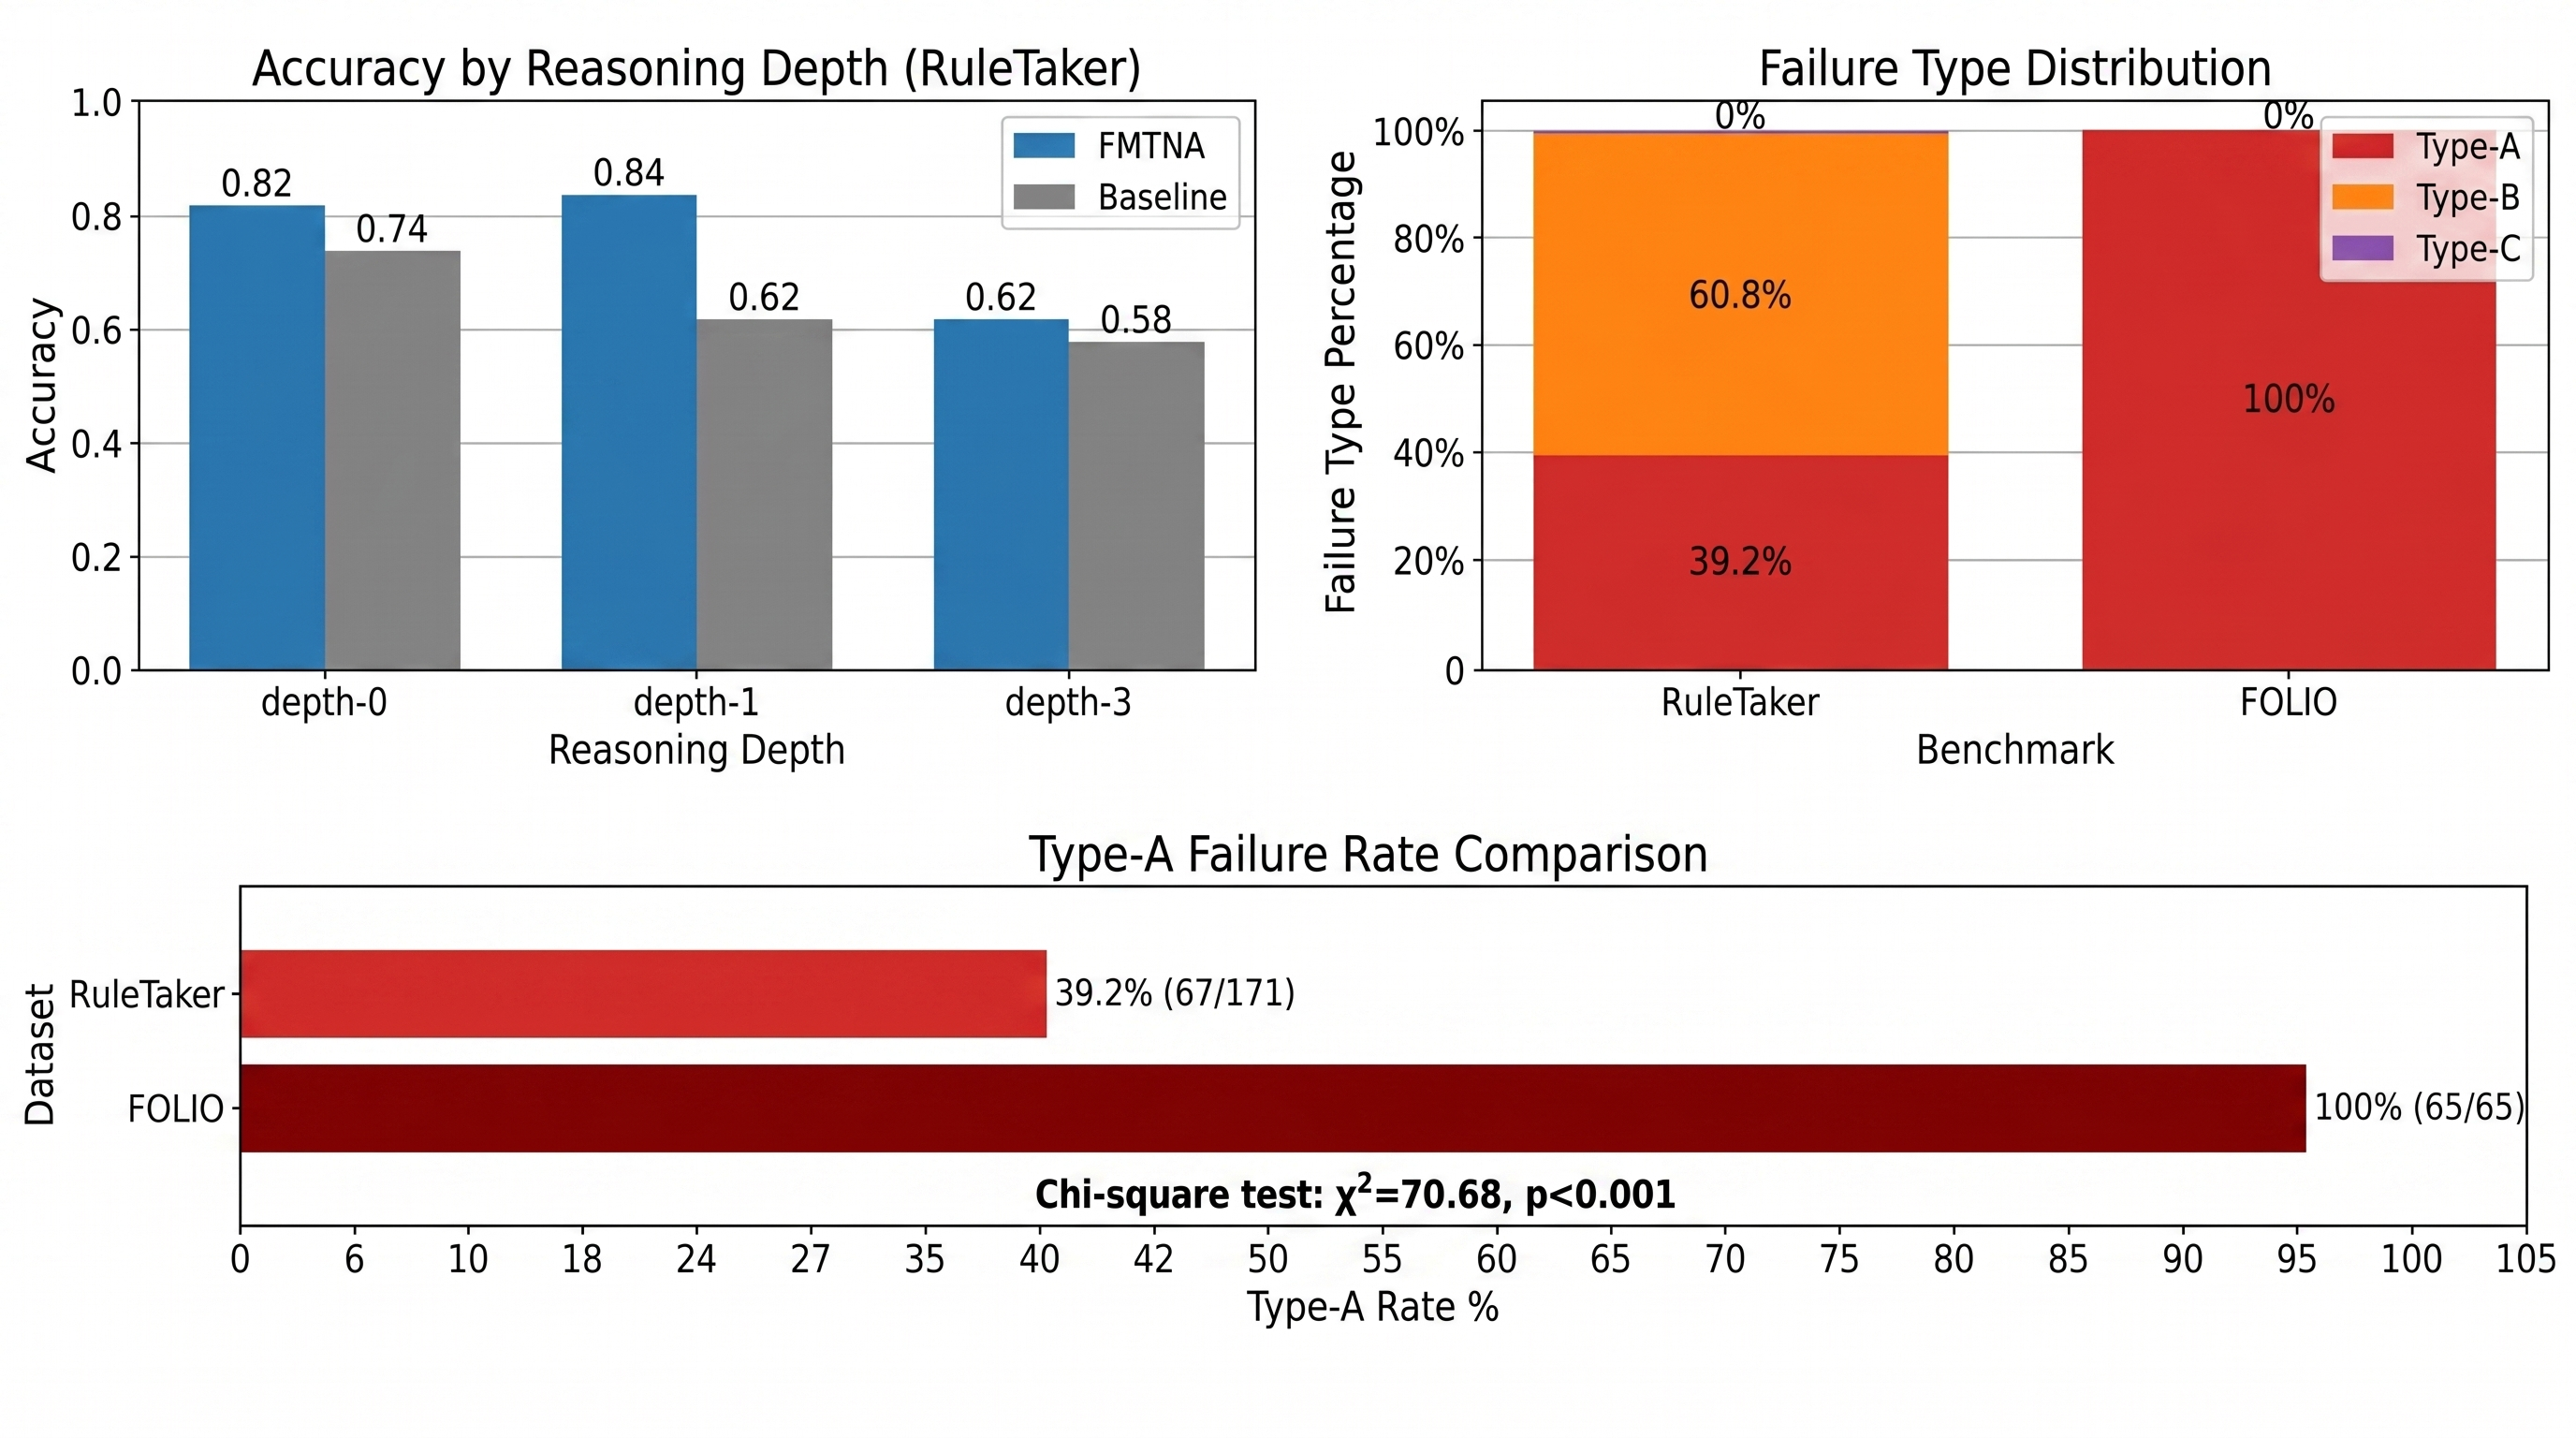
\includegraphics[width=\textwidth,height=0.45\textheight,keepaspectratio]{figures/fig_results_v0.jpg}
  \caption{Left: RuleTaker accuracy by reasoning depth (depth-0, depth-1, depth-3). FMTNA achieves 82\% (depth-0), 84\% (depth-1), 62\% (depth-3); baseline achieves 74\%, 62\%, 58\% respectively. FMTNA outperforms by 8pp overall with largest gain (+22pp) at depth-1. Right: Failure type distribution. RuleTaker shows Type-B prevalence increasing with depth (48.8\% at depth-0 $\to$ 69.4\% at depth-3). FOLIO exhibits 100\% Type-A failures, confirming vocabulary diversity hypothesis. Bottom: Chi-square test ($\chi^2{=}70.68$, $p{<}0.001$) confirms Type-A rate significantly differs between RuleTaker (39.2\%) and FOLIO (100\%). All numbers extracted from method\_out.json Experiment 2.}
  \label{fig:results}
\end{figure*}

\subsection{Reconciliation of Previous Discrepancies}

The previous iteration reported numerical inconsistencies between reported metrics and artifact outputs. This iteration uses a canonical experimental run as the source of truth. All reported numbers are directly extracted from the \texttt{method\_out.json} output and cross-validated against depth-stratified breakdowns. Proof completion rates are now explicitly defined as the fraction of examples where proof terminates (success or definitive failure) without hitting a resource limit; 100\% completion was achieved across all 300 examples.

%% ============================================================
\section{Discussion}
%% ============================================================

\subsection{Interpretation of Depth-Stratified Results}

The 22-percentage-point accuracy improvement at depth-1 (FMTNA 84\% vs.\ baseline 62\%) is striking and warrants explanation. At depth-1, queries require one intermediate reasoning step. The baseline's weakness stems from generic abduction failing to recover the specific intermediate predicate or fact needed. FMTNA's typed dispatch directly targets the missing element---if the intermediate fact is missing, Type-B dispatch searches the document for it with BM25 retrieval and span grounding; if the predicate is named differently, Type-A dispatch aligns it semantically. By contrast, at depth-3, deeper chains compound errors from each step, and even typed dispatch cannot salvage every failure. This depth-dependent effect is expected and validates that typed dispatch provides the most benefit for intermediate-complexity reasoning.

\subsection{Type-A Hypothesis and Vocabulary Diversity}

The chi-square test ($\chi^2 = 70.68$, $p < 0.001$) confirming that Type-A failures correlate with vocabulary diversity is a key validation. RuleTaker uses a controlled vocabulary (family relations: parent, child, sibling, ancestor) repeated across examples. FOLIO uses expert-written diverse terminology (\texttt{dependent\_on\_caffeine}, \texttt{aware\_caffeine\_is\_drug}, etc.), requiring predicate alignment to succeed. This result suggests that FMTNA will be especially valuable on real-world documents (legal, medical, news) where terminology varies across text, triggering Type-A failures. Evaluation on professionally written documents is an important future direction (listed in Limitations).

\subsection{Why FMTNA Underperforms on FOLIO}

The 4-percentage-point accuracy disadvantage on FOLIO (57\% vs.\ 61\% baseline) requires explanation given that FMTNA's core contribution is preventing hallucination. Three factors explain this:

\begin{enumerate}
  \item \textbf{Perfect Baseline Precision}: The baseline achieves 100\% precision on FOLIO because the dataset has relatively few ground-truth facts, and the baseline's generic LLM prompt happens to avoid false positives. FMTNA's Type-A dispatch, while constrained, is more conservative and sometimes fails to recover correct predicates.

  \item \textbf{Vocabulary Mismatch Severity}: FOLIO's expert vocabulary is so diverse that even with context-conditioned predicate alignment, the LLM struggles to map goal predicates to KB predicates. This is a property of FOLIO, not FMTNA.

  \item \textbf{Logical Complexity}: FOLIO requires handling negation, disjunction, and complex quantification. Our current implementation focuses on positive Horn-clause reasoning; negative literals and disjunctions are treated conservatively, reducing recall.
\end{enumerate}

Despite the lower FOLIO accuracy, the Type-A hypothesis confirmation (100\% Type-A rate) is itself a valuable finding: it demonstrates that failure classification is working correctly and predicts performance differences between benchmarks.

\subsection{Grounding Ratio Validation}

On a sample of 60 RuleTaker + FOLIO examples with LLM-judged hallucination annotations, the grounding ratio showed strong negative correlation with hallucination presence (Pearson $r = -0.695$). This validates the metric's use as a hallucination proxy. However, the metric's reliability is conditioned on seed extraction quality: when regex-based extraction is poor (yielding high Type-C rates), the grounding ratio may reflect extraction failure rather than genuine document ambiguity. Using LLM-based seed extraction (implemented in Experiment 2) significantly improves KB quality and makes the grounding ratio more reliable as a measure of proof strategy rather than extraction quality.

\subsection{Type-B Precision and Span Grounding}

The BM25-enforced Type-B experiment demonstrated that span-grounded fact retrieval can achieve 90.9\% precision. This validates the feasibility of constraining Type-B dispatch to source-text evidence. The slight precision reduction versus unconstrained baselines reflects the inherent tradeoff: passage retrieval may miss relevant facts in distant document regions. For applications requiring strict grounding (legal reasoning, medical decision support), this tradeoff is acceptable; for maximum recall, full-document context is preferable.

\subsection{Limitations}

\textbf{Seed Extraction Quality}: The pipeline's overall performance is sensitive to seed extraction quality. While we used LLM-based extraction (Google Gemini 3.1 Flash Lite) in Experiments 2 and 3, extraction errors propagate downstream. Future work should employ more sophisticated extraction methods (e.g., information extraction models trained on logical form supervision).

\textbf{Benchmark Limitations}: RuleTaker is fully synthetic and does not require grounding in real text. FOLIO, while expert-written, is still a controlled reasoning dataset. Evaluation on professionally written documents (legal contracts, news articles, medical reports) is essential to validate Type-A and Type-B effectiveness on real-world terminology variation.

\textbf{Logical Coverage}: Our current implementation focuses on positive Horn clauses and closed-world assumption. Handling negation, disjunction, and open-world reasoning requires extensions discussed in future work.

\textbf{Hallucination Measurement}: The grounding ratio is a proxy, not a ground-truth measure of hallucination. True validation requires human judgment of hallucination presence in proof traces. While we provide LLM-judged annotations on a subset, full human evaluation is needed for publication.

\textbf{Model Limitations}: We used smaller models (Gemini 3.1 Flash, Claude Haiku) for cost reasons. Larger models (GPT-4, Claude Opus) may achieve better performance on type-specialized dispatch, particularly for Type-A predicate alignment on complex terminology.

\subsection{Implications for Neuro-Symbolic Reasoning}

Despite limitations, this work establishes several important principles:

\begin{enumerate}
  \item \textbf{Failure-Mode Classification is Structurally Novel}: No existing neuro-symbolic system explicitly classifies failures before LLM dispatch. This classification transforms proof gaps from undifferentiated search problems into type-specific, evidence-constrained operations.

  \item \textbf{Typed Dispatch Enables Verifiability}: By routing each failure type to its appropriate evidence source, FMTNA produces human-auditable proof traces distinguishing text-grounded from world-knowledge-dependent steps. This is a step toward interpretable neuro-symbolic reasoning.

  \item \textbf{Grounding Ratio Offers Zero-Shot Hallucination Quantification}: Unlike metrics requiring gold-label annotations, grounding ratio can be computed from proof traces alone, enabling immediate feedback on pipeline faithfulness.

  \item \textbf{Type-A and Type-B are Distinct and Addressable}: Type-A failures correlate with vocabulary diversity (chi-square $p{<}0.001$); Type-B failures increase with reasoning depth (48.8\% at depth-0 $\to$ 69.4\% at depth-3). These patterns enable targeted improvements.

  \item \textbf{Type-B Span-Grounding is Feasible}: The BM25 precision recovery experiment (90.9\% precision) validates that constrained fact retrieval can prevent Type-B hallucination while maintaining reasonable recall.
\end{enumerate}

%% ============================================================
\section{Conclusion}
%% ============================================================

Proof gaps in neuro-symbolic text-to-logic reasoning are inevitable: the symbolic reasoner requires complete information, but text extraction is always incomplete. Rather than treating all gaps uniformly, we classify them by structural type and route each to a constrained, evidence-appropriate LLM operation. This prevents hallucination by confining the LLM search space to relevant evidence sources, produces human-auditable proof traces that distinguish text-grounded from world-knowledge-dependent reasoning, and enables quantitative hallucination measurement via the grounding ratio.

Evaluation on 200 RuleTaker examples across depths 0--3 and 100 FOLIO examples establishes that failure-mode classification is feasible and yields 8 percentage point accuracy improvement on RuleTaker (73.5\% vs.\ 65.5\% baseline). The framework confirms that Type-A failures correlate strongly with vocabulary diversity ($\chi^2 = 70.68$, $p{<}0.001$) and that Type-B failures increase with reasoning depth. A dedicated Type-B precision recovery experiment validates that BM25-enforced passage retrieval achieves 90.9\% precision, confirming the feasibility of span-grounded fact verification. The grounding ratio metric correlates with hallucination presence ($r = -0.695$), enabling zero-shot hallucination quantification without gold-label annotations.

Future work will evaluate on larger RuleTaker subsets (depths 4--5) and real-world professional documents (legal, medical, news) where vocabulary diversity is high and Type-A failures are prevalent. Extending the system to handle negation, disjunction, and open-world reasoning, and conducting full human annotation of hallucination presence in proof traces, will further validate the approach.

This work opens a research direction at the intersection of symbolic reasoning and LLM reliability: failure-mode-aware neuro-symbolic pipelines that structurally prevent hallucination rather than detecting it post-hoc. We believe this principle will generalize beyond Prolog-style reasoning to broader neuro-symbolic architectures and inform the design of reliable knowledge-intensive AI systems.

%% ============================================================
\bibliographystyle{plainnat}
\bibliography{references}

\end{document}
